%%%%%%%%%%%%%%%%%%%%%%%%%%%%%%%%%%%%%%%%%
% Journal Article
% LaTeX Template
% Version 1.0 (25/8/12)
%
% This template has been downloaded from:
% http://www.LaTeXTemplates.com
%
% Original author:
% Frits Wenneker (http://www.howtotex.com)
%
% License:
% CC BY-NC-SA 3.0 (http://creativecommons.org/licenses/by-nc-sa/3.0/)
%
%%%%%%%%%%%%%%%%%%%%%%%%%%%%%%%%%%%%%%%%%

%----------------------------------------------------------------------------------------
%	PACKAGES AND OTHER DOCUMENT CONFIGURATIONS
%----------------------------------------------------------------------------------------

\documentclass[twoside]{article}

% rajout personnel
\usepackage{graphicx}

\usepackage{lipsum} % Package to generate dummy text throughout this template

\usepackage[sc]{mathpazo} % Use the Palatino font
\usepackage[T1]{fontenc} % Use 8-bit encoding that has 256 glyphs
\linespread{1.05} % Line spacing - Palatino needs more space between lines
\usepackage{microtype} % Slightly tweak font spacing for aesthetics

\usepackage[hmarginratio=1:1,top=32mm,columnsep=20pt]{geometry} % Document margins
\usepackage{multicol} % Used for the two-column layout of the document
\usepackage{hyperref} % For hyperlinks in the PDF

\usepackage[hang, small,labelfont=bf,up,textfont=it,up]{caption} % Custom captions under/above floats in tables or figures
\usepackage{booktabs} % Horizontal rules in tables
\usepackage{float} % Required for tables and figures in the multi-column environment - they need to be placed in specific locations with the [H] (e.g. \begin{table}[H])

\usepackage{lettrine} % The lettrine is the first enlarged letter at the beginning of the text
\usepackage{paralist} % Used for the compactitem environment which makes bullet points with less space between them

\usepackage{abstract} % Allows abstract customization
\renewcommand{\abstractnamefont}{\normalfont\bfseries} % Set the "Abstract" text to bold
\renewcommand{\abstracttextfont}{\normalfont\small\itshape} % Set the abstract itself to small italic text

\usepackage{titlesec} % Allows customization of titles
\titleformat{\section}[block]{\large\scshape\centering{\Roman{section}.}}{}{1em}{} % Change the look of the section titles 

\usepackage{fancyhdr} % Headers and footers
\pagestyle{fancy} % All pages have headers and footers
\fancyhead{} % Blank out the default header
\fancyfoot{} % Blank out the default footer
\fancyhead[C]{Bayesian Networks $\bullet$ October 2012} % Custom header text
\fancyfoot[RO,LE]{\thepage} % Custom footer text

%----------------------------------------------------------------------------------------
%	TITLE SECTION
%----------------------------------------------------------------------------------------

\title{\vspace{-15mm}\fontsize{24pt}{10pt}\selectfont\textbf{Bayesian networks}} % Article title

\author{
\large
\textsc{Philippe Pittoli}\\[2mm] % Your name
\normalsize University of Strasbourg \\ % Your institution
\normalsize \href{mailto:philippe.pittoli@etu.unistra.fr}{contact-me} % Your email address
\vspace{-5mm}
}
\date{}

%----------------------------------------------------------------------------------------

\begin{document}

\maketitle % Insert title

\thispagestyle{fancy} % All pages have headers and footers

%----------------------------------------------------------------------------------------
%	ARTICLE CONTENTS
%----------------------------------------------------------------------------------------

%\begin{multicols}{1} % Two-column layout throughout the main article text

\section{A simple explanation of Bayesian networks}

%\lettrine[nindent=0em,lines=3]{L} orem ipsum dolor sit amet, consectetur adipiscing elit.
%\lipsum[2-3] % Dummy text
Bayesian network is based on the Bayes' theorem that we have already talked about in class.
This model is probabilistic and is mainly used in data mining, in medical and industrial diagnostics and in spam detection.
This Bayesian or "belief" network aims at showing conditional probability and causality relationships between variables.
The variables can be events, or states.
What is called "conditional probability" is the probability of an event occuring given that another event has occurred.

We can find some representations of this kind of networks (acyclic graphs) on the internet, like this one :

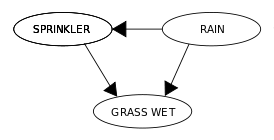
\includegraphics{SimpleBayesNetNodes.png}

The circles are called "nodes" and contain the variable name.
There are links (arrows) between them, which are called "arcs" and they indicate a dependency. 
In a Bayesian network, only the variables without arrows are independent.
On this figure (from Wikipedia), we can see the "sprinkler" event which is the child of the variable "rain".
The "grass wet" event is caused by one (or more) of its parents.
Thanks to this graph, we can make a table with the probability of an event to occur or not given the fact that another event occurred before or not.
The grass has a great probability of being wet if the event "rain" occurs, less if it doesn't.

The graph is the first step in the construction of a Bayesian network, 
then we can take statistics to determinate a table of probabilities for each variable from the structure, 
according to its dependencies.


%------------------------------------------------


%\end{multicols}

\end{document}
